\chapter{Aleatoriedade}

A aleatoriedade é um conceito fundamental em diversas disciplinas, sendo
essencial entender o que ela realmente é. Aleatoriedade é vital em diversas
aplicações, sobretudo em áreas como criptografia, simulações computacionais e
teoria da informação. No entanto, quando lidamos com computadores, a produção
de números verdadeiramente aleatórios é um desafio intrínseco. Em geral, os
números gerados por algoritmos computacionais são \emph{pseudo-aleatórios},
ou seja, seguem sequências determinísticas que apenas aparentam não possuir uma
ordem subjacente. Esses números são o resultado de funções matemáticas bem
definidas, como geradores lineares congruentes ou algoritmos mais sofisticados,
como o Mersenne Twister, que, apesar de produzirem sequências com propriedades
estatísticas desejáveis, carecem da imprevisibilidade essencial à aleatoriedade
genuína.

Stephen Wolfram, renomado por suas contribuições à complexidade computacional e
à teoria dos sistemas complexos, propõe três fontes distintas de aleatoriedade
que explicam como ela pode emergir em sistemas: a aleatoriedade do ambiente, a
aleatoriedade nas condições iniciais e a geração intrínseca de aleatoriedade. A
\emph{aleatoriedade do ambiente} surge de influências externas imprevisíveis,
como variações naturais em sistemas climáticos, que injetam incerteza contínua
em um sistema. A \emph{aleatoriedade nas condições iniciais} reflete a
sensibilidade de sistemas caóticos a pequenas perturbações iniciais,
exemplificada pelo ``efeito borboleta'', onde mudanças mínimas podem levar a
resultados drasticamente distintos. Já a \emph{geração intrínseca de
aleatoriedade} ocorre nas dinâmicas internas de sistemas determinísticos
complexos, que, por meio de interações não-lineares, produzem comportamentos
aparentemente aleatórios, como o ruído quântico em circuitos eletrônicos.
Wolfram argumenta que essas fontes frequentemente coexistem, e, em suas
palavras, até ``programas simples podem produzir comportamento aparentemente
aleatório mesmo sem entrada aleatória alguma'', sugerindo que os mecanismos
subjacentes à aleatoriedade na natureza e em simulações computacionais
compartilham uma essência comum \parencite{wolfram2002}.

Fontes de aleatoriedade genuína, por outro lado, frequentemente recorrem ao
mundo físico, indo além dos métodos algorítmicos determinísticos. Exemplos
clássicos incluem o ruído térmico em circuitos eletrônicos, a decadência
radioativa ou fenômenos atmosféricos captados por sensores, usados em geradores
de números aleatórios baseados em hardware. Em sistemas computacionais
modernos, busca-se capturar essa aleatoriedade verdadeira por meio de eventos
imprevisíveis do ambiente operacional, como os pressionamentos de teclas no
teclado, os movimentos do mouse, as variações no tráfego de rede, a velocidade
das ventoinhas do processador, o ruído de acesso a discos rígidos ou até mesmo
as flutuações nos tempos de execução de processos do sistema. Esses dados,
coletados em tempo real, são usados como sementes ou entradas diretas para
aumentar a imprevisibilidade dos números gerados.
Contudo, essas abordagens enfrentam limitações práticas, pois dependem de
sistemas computacionais determinísticos que podem comprometer a coleta e o uso
desses dados brutos ao processá-los de maneira previsível.

Um exemplo prático disso é encontrado no sistema operacional Linux, que utiliza
duas fontes principais de números aleatórios: \texttt{/dev/random} e
\texttt{/dev/urandom}. O dispositivo \texttt{/dev/random} gera números
aleatórios de alta qualidade a partir de uma ``piscina de entropia'' alimentada
por ruído ambiente, como os eventos mencionados, mas pode bloquear a leitura se
a entropia disponível for insuficiente, tornando-o ideal para operações
criptográficas que priorizam segurança sobre velocidade. Já o
\texttt{/dev/urandom}, embora também utilize a mesma piscina de entropia, não
bloqueia a leitura, gerando dados adicionais mesmo em baixa entropia ao
reutilizar e estender os valores coletados; isso o torna mais adequado para
aplicações como simulações, que demandam grandes quantidades de números
aleatórios rapidamente.

\section{O Gerador Lehmer}

Um dos primeiros métodos métodos proposto para gerar números aleatórios é o método de Lehmer,
proposto por Derrick Henry Lehmer na década de 1940. O método se baseia em uma
relação de recorrência linear para produzir sequências de valores aparentemente
aleatórios. Esse gerador, frequentemente classificado como um Gerador Linear
Congruencial, utiliza a multiplicação e o módulo como peças fundamentais, definindo
cada novo número na sequência por meio de:
\begin{equation}
  X_{k+1} = g \cdot X_k \mod n ,
\end{equation}
onde $X_k$ é o estado atual, $g$ é um multiplicador (idealmente uma raiz primitiva módulo $n$),
$n$ é o módulo (geralmente um número primo ou potência de um primo), e $X_0$ é a semente inicial,
que deve ser coprima com $n$. 

Apesar de sua simplicidade, o Gerador Lehmer revela questões importantes sobre a
percepção de aleatoriedade, tema que explorado por Stephen Wolfram em seus
estudos sobre sistemas complexos. Wolfram demonstrou que a aparente
aleatoriedade de uma sequência pode variar dramaticamente dependendo de como
ela é visualizada. Por exemplo, ao representar os números gerados por um gerador linear congruencial
como uma sequência unidimensional de valores, a saída pode parecer caótica e
desprovida de padrões. No entanto, ao organizá-los em uma matriz
bidimensional --- onde cada valor é plotado como um ponto em linhas e colunas
--- ou mesmo em um cubo tridimensional, estruturas subjacentes, como repetições
ou diagonais, podem emergir, revelando a natureza determinística do processo.
A \Cref{fig:lehmer} ilustra um exemplo utilizando $g=3$ e $n=2^{32}$.
\begin{figure}
  \centering
  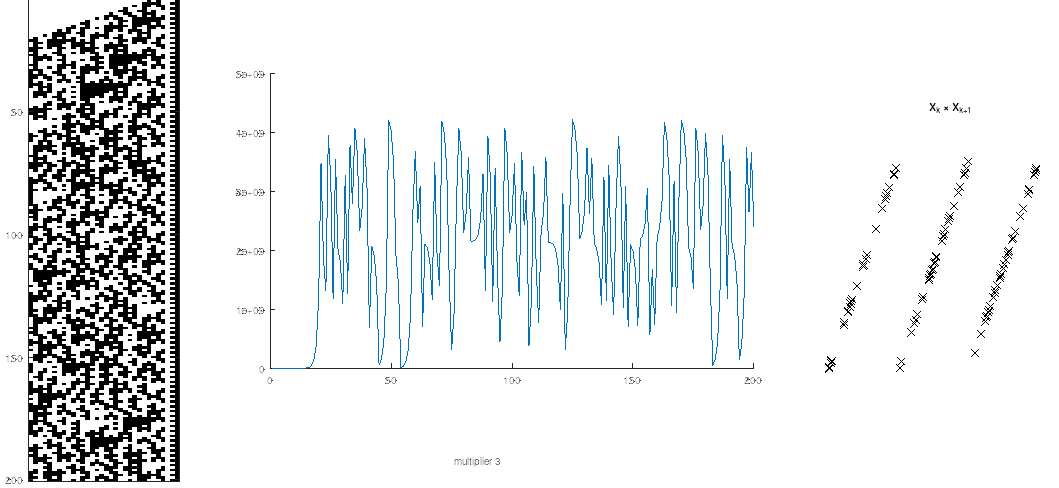
\includegraphics[width=\linewidth]{plots/lehmer.png}
  \caption{Representação da sequência de 200 números gerados pelo gerador Lehmer.
  À esquerda, a representação binárias dos números, no meio um gráfico da sequência e,
  por fim, a representação de $X_k \times X_{k+1}$.}\label{fig:lehmer}
\end{figure}
Esse fenômeno também ocorre na Regra 30 proposta por Wolfram,
onde uma simples regra iterativa gera saídas que parecem aleatórias em uma dimensão, mas exibem ordem
em representações visuais alternativas.

A relação entre aleatoriedade e visualização no contexto do Gerador Lehmer
destaca suas limitações práticas. Se os parâmetros $g$ e $n$ forem mal
escolhidos, a sequência pode apresentar ciclos curtos ou padrões visíveis,
comprometendo sua utilidade em aplicações que exigem alta imprevisibilidade.
Por exemplo, em testes gráficos como o plano de fases (plotando $X_k$ contra
$X_{k+1}$), geradores lineares simples frequentemente revelam retas ou grades,
evidenciando correlações indesejadas. Mesmo com parâmetros otimizados, a
natureza determinística do método implica que ele nunca produz aleatoriedade
genuína, apenas uma aproximação que pode ser suficiente para cenários, como
simulações básicas, mas inadequada para criptografia.




\section{O Gerador Mersenne Twister}

O Mersenne Twister é um algoritmo de geração de números pseudoaleatórios
desenvolvido por Makoto Matsumoto e Takuji Nishimura em 1997, amplamente
reconhecido por sua capacidade de produzir sequências com propriedades
estatísticas de alta qualidade e um período excepcionalmente longo. O nome
``Mersenne Twister'' reflete sua fundamentação matemática: o algoritmo utiliza
números primos de Mersenne --- números primos da forma $2^p - 1$, onde $p$ é
também um primo --- e emprega uma técnica chamada \textit{twisting} para
garantir a geração de números com boa distribuição estatística e independência
aparente. O algoritmo é projetado para prover uma distribuição uniforme e baixa
correlação entre valores consecutivos.

O Mersenne Twister também oferece um equilíbrio entre qualidade estatística e
eficiência computacional. Embora não seja o gerador mais rápido disponível ---
métodos mais simples, como geradores lineares congruenciais, podem ser mais
rápidos em termos de tempo de execução ---, ele compensa com sua robustez e
confiabilidade, tornando-o adequado para uma ampla gama de aplicações. Por essa

O Mersenne Twister também possui uma boa eficiência computacional, sendo por
isso amplamente adotado em linguagens de programação, como a função
\texttt{rand} do Octave e do MATLAB, que utiliza a variante MT19937 com período
$2^{19937} - 1$ (seu período extremamente longo), bem como em bibliotecas
padrão de linguagens como Python (\texttt{random}) e C++
(\texttt{std::mt19937}). Apesar de suas qualidades, o Mersenne Twister é
inadequado para aplicações criptográficas.


\subsection{MT19937}

O Mersenne Twister (MT)~\parencite{matsumoto1998mersenne} é um dos geradores de
números pseudoaleatórios (RNGs) mais amplamente utilizados, sendo um GFSR
(\textit{Generalized Feedback Shift Register}) com \textit{twist}.
Conforme \textcite{tan2016}, o algoritmo
do MT pode ser descrito pelas seguintes etapas:

\begin{itemize}
    \item \textbf{Inicialização:} Defina $r$ números de $w$ bits $(x_i, i = 1, 2, \ldots, r)$ aleatoriamente como valores iniciais.
    \item \textbf{Definição da Matriz de Recorrência:} Considere a matriz
    \[
    A = \begin{pmatrix}
    0 & I_{w-1} \\
    a_w & a_{w-1} \cdots a_1
    \end{pmatrix},
    \]
    onde $I_{w-1}$ é a matriz identidade $(w-1) \times (w-1)$, e $a_i, i = 1, \ldots, w$, assume valores 0 ou 1.
    \item \textbf{Recorrência:} Para cada $i \geq 0$, calcule
    \[
    x_{i+r} = (x_{i+s} \oplus (x_i^{(w:(l+1))} | x_{i+1}^{(l:1)}) A),
    \]
    onde $x_i^{(w:(l+1))}| x_{i+1}^{(l:1)}$ representa a concatenação dos $w-l$ bits mais significativos (superiores)
    de $x_i$, e $x_{i+1}^{(l:1)}$ os $l$ bits menos significativos de $x_{i+1}$.
    \item \textbf{Tempering:} Para cada $x_{i+r}$, aplique as operações sequencialmente:
    \[
    \begin{aligned}
    z &= x_{i+r} \oplus (x_{i+r} \gg t_1), \\
    z &= z \oplus ((z \ll t_2) \land m_1), \\
    z &= z \oplus ((z \ll t_3) \land m_2), \\
    z &= z \oplus (z \gg t_4), \\
    u_{i+r} &= z / (2^w - 1),
    \end{aligned}
    \]
    onde $t_1, t_2, t_3, t_4$ são inteiros, $m_1, m_2$ são máscaras de bits, 
    e $\land$ é a operação \textit{bitwise AND}. Os valores $u_{i+r}, i = 1, 2, \ldots$, 
    formam a sequência no intervalo $[0, 1]$.
\end{itemize}

Com valores apropriados de $r$, o MT pode gerar sequências com período de até
$2^{19937}$, além de possuir boas propriedades
estatísticas \parencite{matsumoto1998mersenne}.






\subsection{Abordagens para Geração de Números Pseudoaleatórios}

Diversas abordagens existem para gerar números pseudoaleatórios
\parencite{knuth1997art,matsumoto1998mersenne,wolfram2002,kocarev2011chaos,kneusel2018random},
abaixo listamos algumas delas:

\begin{itemize}
    \item Geradores Lineares Congruenciais (LCGs): \\
	Baseiam-se em uma relação de recorrência linear da forma 
	\begin{equation}
	    X_{n+1} = (a \cdot X_n + c) \mod m ,
	\end{equation} 
	como o exemplo do Gerador Lehmer visto anteriormente.
	Este tipo de gerador é simples, mas com período curto e baixa qualidade estatística.
    \item Geradores de Fibonacci com Atraso (LFGs): \\
	Geram números combinando valores anteriores da sequência usando uma operação (como adição ou XOR) com atrasos:
	\begin{equation}
	    X_n = (X_{n-k} \oplus X_{n-l}) \mod 2^w ,
	\end{equation} 
	oferecendo períodos longos, mas exigindo estados iniciais grandes.
    \item Autômatos Celulares: \\ 
	Aplicam regras como a Regra 30 vista anteriormente, 
	\begin{equation} 
	    c_i(t+1) = c_{i-1}(t) \oplus (c_i(t) \lor c_{i+1}(t)) ,
	\end{equation} 
	gerando padrões caóticos, porém computacionalmente custosos.
    \item Funções de Hash e Criptográficas: \\
	Utilizam funções como SHA-256 ($R_i = H(S || C)$) ou cifras de fluxo como ChaCha ($R_i = \text{ChaCha}(K, C)$), 
	sendo seguras para criptografia, porém mais lentas.
    \item Geradores Baseados em Caos: \\
	Empregam sistemas caóticos, como o mapa logístico 
	\begin{equation}
	    X_{n+1} = r \cdot X_n \cdot (1 - X_n) ,
	\end{equation}
	com comportamento caótico, mas sensíveis a precisão numérica.
\end{itemize}

